\documentclass[12pt,a4paper]{article}

\usepackage[UTF8]{ctex}
\usepackage[backend=bibtex]{biblatex}
\usepackage{amsmath,amsthm,amssymb,graphicx,multirow,float,caption}
\usepackage{geometry}
\geometry{left=2.54cm, right=2.54cm, top=3.18cm, bottom=3.18cm}
\usepackage{enumitem}
\usepackage{subcaption,booktabs,diagbox}
\setenumerate[1]{itemsep=0pt,partopsep=0pt,parsep=\parskip,topsep=5pt}
\setitemize[1]{itemsep=0pt,partopsep=0pt,parsep=\parskip,topsep=5pt}
\setdescription{itemsep=0pt,partopsep=0pt,parsep=\parskip,topsep=5pt}
\usepackage{adjustbox}
\usepackage[graphicx]{realboxes}
\usepackage{rotating}
\usepackage{parskip}
\usepackage{titlesec}
\usepackage{pdfpages}
\newcommand{\be}[1]{
    \begin{equation}
        #1
    \end{equation}
}

\newcommand{\bfig}[3]{
    \begin{figure}[H]
        \centering
        \includegraphics[width=#1\textwidth]{#2}
        \caption{#3}
    \end{figure}
}

\titleformat{\section}%设置section的样式
{\raggedright\large\bfseries}%右对齐,4号字,加粗
{\thesection .\quad}%标号后面有个点
{0pt}%sep label和title之间的水平距离
{}%标题前没有内容

\title{\vspace{-4cm}\Large 非线性电路混沌及同步控制}  %文章标题
\author{\kaishu 学号:202111030007 \hspace{2cm} 姓名:郑晓旸}   %作者的名称
\date{}

\begin{document}
\maketitle

\begin{abstract}
    本实验利用有源非线性负阻为主要载体, 测量并且得到了非线性负阻的
I-U 曲线, 并分段进行了线性拟合, 分段得到了 I-U 函数关系, 并确定了负阻
区。
并利用经典的非线性电路——蔡氏电路, 通过相图研究了倍周期分岔通往
混沌这一典型路径, 观察系统在该路径下的不同状态, 并因此得到了不同状态
对应非线性电阻的工作区。后利用电容箱测量了费根鲍姆常数。
利用隔离器在两个蔡氏电路的之间实现了单向映射, 并依此成功完成了混
沌同步的实验, 观察了两个系统之间的混沌同步, 准同步, 去同步现象。
最后在混沌同步电路的基础上, 模拟了加密通信的过程, 进行了混沌加密通
信实验, 并且可得到较为清晰的解密信号。

\bf{关键词: 非线性负阻\quad 费根鲍姆常数\quad 混沌同步}
\end{abstract}

\section{引言}
混沌性是非线性动力学特有的运动形式, 它是由确定性系统产生的随机现象. 确定性是说, 系统的动力学方程是确定的. 随机性是说, 系统演化过程中的任何微小扰动都会在长时间发展中带来完全不同的结果, 
即蝴蝶效应. 但需要注意, 这种随机性是系统的内在性质, 混沌不同于无序. 

本实验将通过电路系统观察混沌系统. 该电路的核心是一种有源非线性电阻, 并通过蔡氏电路, 可以精密地改变实验条件得到丰富的实验结果. 

本实验的目的是学习有源非线性负阻元件的工作原理,借助蔡氏电路掌握非线性动力学系统运
动的一般规律,了解混沌同步和控制的基本概念,了解混沌通信原理。通过本实验的学习扩展视野、
活跃思维,以一种崭新的科学世界观来认识事物发展的规律。

\section{原理}
\subsection{倍周期分岔与费根鲍姆常数}
非线性系统中同时具有周期性和混沌性. 通过改变参量$\mu$, 系统从定态(即每个周期的运动状态完全一致)出发, 由倍周期分叉通向混沌. 其结果是系统的周期数目不断加倍, 从定态的P变为2P继而为4P以致于为$2^n P$, 直至出现混沌. 在一个$2^n P$的混沌周期运动中, 每一P时间段内的运动既相似又不同, 在相平面内显示为分叉. 费根鲍姆发现, 
在倍周期分叉点的系统参量$\mu$的取值$\mu_{n}$将呈现收敛: 
\be{\delta_{n}=\frac{\mu_{n}-\mu_{n-1}}{\mu_{n+1}-\mu_{n}}\rightarrow 4.6992016091029...}

\subsection{有源非线性电阻}
非线性元件的I-U曲线是非线性的, 如果$\frac{dI}{dU}<0$, 就是出现了负的微分电阻. 从能量的角度来说, 负阻与正阻不同, 正阻消耗功率, 负阻向外界输出功率.

实验中采用的非线性负阻, 是由正阻和运算放大器构成的负阻变换电路, 其伏安特性具有三段分段线性的特征. 
\subsection{蔡氏振荡电路}
蔡氏电路由一个非线性电阻, 电感, 可调电阻R和两个电容器C1, C2构成. 如图所示, L和C2构成一个LC震荡电路, 可调电阻R和电容器C1构成一个移相电路. 
当系统进入稳定的震荡时, 有源负阻电阻抵消损耗电阻R, 并使系统产生非线性现象. 

\bfig{0.5}{蔡氏电路.png}{蔡氏振荡电路}

\subsection{非线性动力学}
根据基尔霍夫定律, 可以写下蔡氏电路的运动方程:
\begin{equation}
\left \{ 
    \begin{aligned}
    C_{1} \frac{\mathrm{d} U_{C_{1}}}{\mathrm{~d} t} & =\frac{1}{R}\left(U_{C_{2}}-U_{C_{1}}\right)-\frac{1}{R_{\mathrm{N}}\left(U_{C_{1}}\right)} U_{C_{1}} \\
    C_{2} \frac{\mathrm{d} U_{C_{2}}}{\mathrm{~d} t} & =\frac{1}{R}\left(U_{C_{1}}-U_{C_{2}}\right)+i_{L} \\
    L \frac{\mathrm{d} i_{L}}{\mathrm{~d} t} & =-U_{C_{2}}
    \end{aligned} 
\right .
\end{equation}
该方程可以用数值方法求解. 利用$U_{C_1}$和$U_{C_2}$绘制X-Y图, 可以观察到倍周期分岔现象. 如图所示:
\bfig{0.8}{倍周期分叉示意图.png}{非线性混沌运动}

图中的运动状态依次是定态1P, 8P, 阵法混沌, 单吸引子, 稳定双吸引子. 
\subsection{混沌同步}
混沌同步是指一个系统的混沌动力学轨道收敛于另一个系统的混沌动力学轨道,以致在以后的
时间里两个系统始终保持
步调一致. 该过程需要两个系统, 一个是用于驱动的混沌系统, 一个是用于响应的子系统. 通过一个由可调电阻控制的单向耦合系统, 可以实现驱动系统对响应系统的单向控制. 

比较两个系统各自的混沌模式图, 以及两个系统中的$U_{C_1}$构成的X-Y图, 可以考察同步情况, 一般分为同步, 准同步和去同步. 
\bfig{0.7}{混沌同步电路.png}{混沌同步电路}

\subsection{混沌通信}
在混沌同步的基础上, 可以实现混沌加密和解密, 并进一步实现混沌通信. 

源端通过加法器将驱动电路的混沌信号与原始信号相加完成加密后传给接收端, 接收端从中减去响应电路的同步信号, 即完成解密. 若有杂波, 需要用滤波器滤去. 

显然, 混沌通信的效果取决于混沌同步的效果. 
\bfig{0.7}{混沌通信电路.png}{混沌通信电路}
\section{实验及结果分析}
\subsection{非线性电阻的伏安特性曲线}
通过改变电阻箱的电阻, 在电压电流快速变化点附近增大采样数, 可得到非线性电阻
的I-U数据曲线如下图所示:
\bfig{0.8}{IU1.png}{实验测量伏安特性曲线}
图中已经包含了拟合结果. 该结果表明, 实验所使用的有源非线性负阻具有三段分段线性的特征. 通过对拟合直线的交点的计算, 可以得到线性区1,2的分段电压U=-1.276V, 线性
区2,3的分段电压为-10.365V. 在-10.365V处达到电流的峰值I=4.92mA. 在U=-12.457V处电流降为0. 

根据拟合结果能看出非线性电阻的I-U曲线并不会经过原点, U=0时I=0.0024mA, 与预期的特
性曲线存在偏差, 可能是非线性电阻外加电源的内阻带来的电压降, 导致非线性元件在路端电压为0时电流不为0. 

将原始数据曲线, 做变换至第二象限, 再旋转180°可得第四象限曲线, 连接第二、四象限曲线得到完
整的非线性负阻I-U特性曲线下图所示: 
\bfig{0.8}{IU2.png}{完整负阻伏安特性曲线}
从图中可以看出, 有效的负阻电压区域为$-10.365V<U<10.365V$. 

\subsection{非线性电路的运动状态}
搭建蔡氏电路, 改变可变电阻R, 观察$U_{C_1}$和$U_{C_2}$的李萨如图, 依照倍周期分岔通往混沌的典型路
径:
$$1P\rightarrow 2P \rightarrow ... 2^n P \rightarrow \text{阵发混沌} \rightarrow \text{周期窗口}(6P,5P,3P)\rightarrow \text{单吸引子}\rightarrow \text{双吸引子}$$

此处的可变电阻是不可视的, 且不能精确控制步长. 实验中在此步骤只能观察到2P, 4P, 3P, 单吸引子, 双吸引子以及中间出现的阵发混沌. 更精细的8P, 5P等, 在下一节调节电容时可以见到. 此处将这些结果一并呈现:

效果如图:
\begin{figure}[H]
    \centering
    \begin{subfigure}[b]{0.3\textwidth}
      \centering
      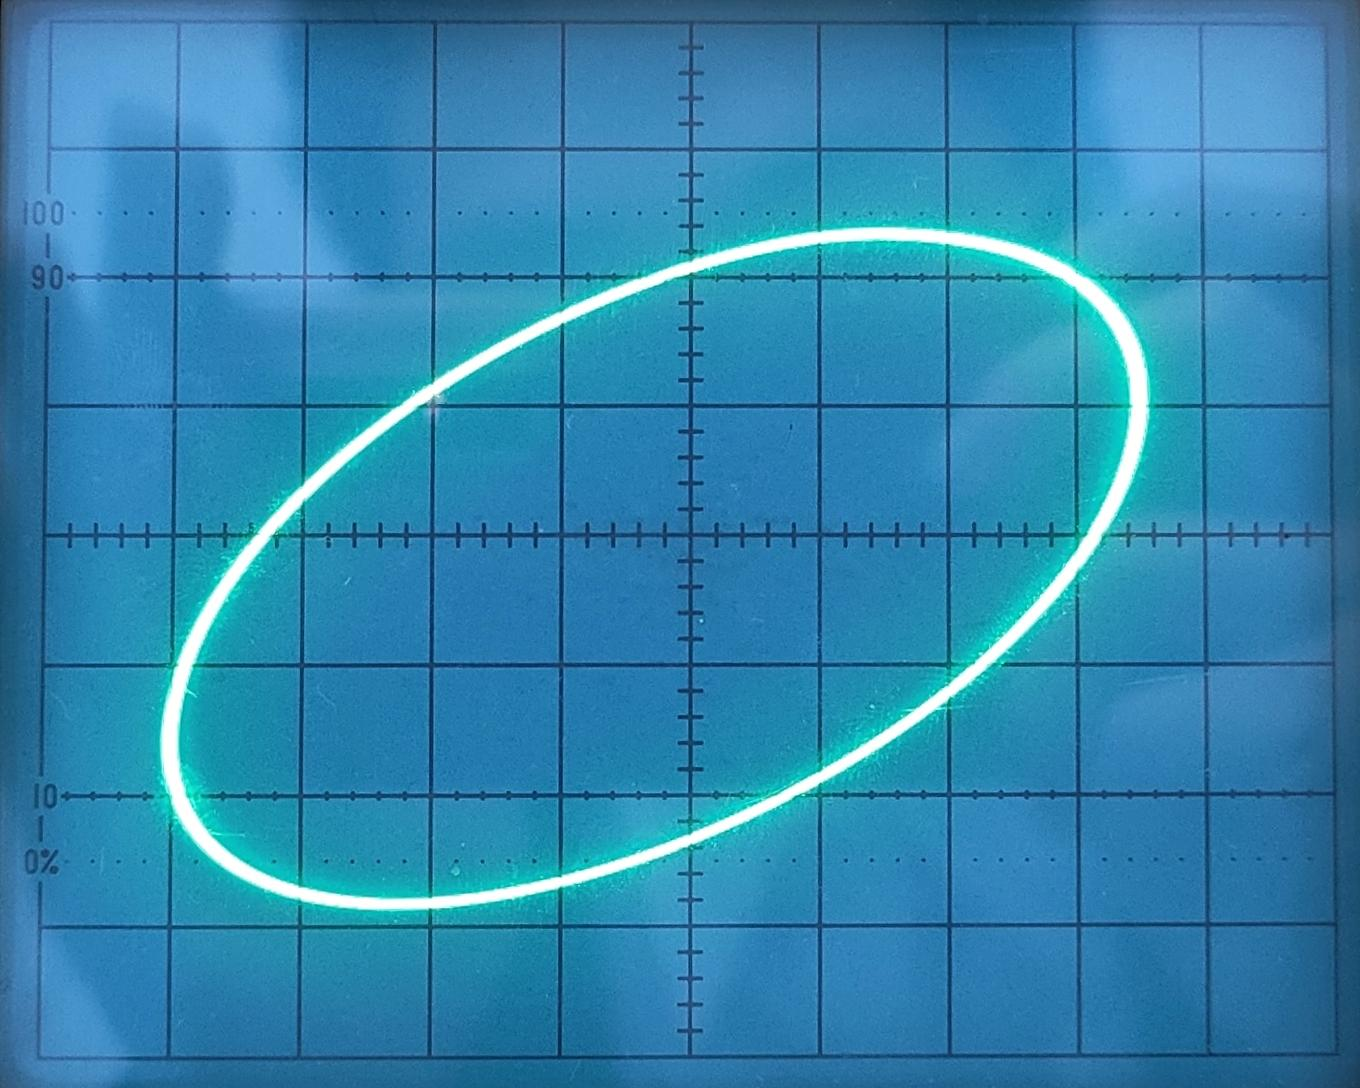
\includegraphics[width=\textwidth]{1P.png}
      \caption{1P}
    \end{subfigure}
    \hfill
    \begin{subfigure}[b]{0.3\textwidth}
      \centering
      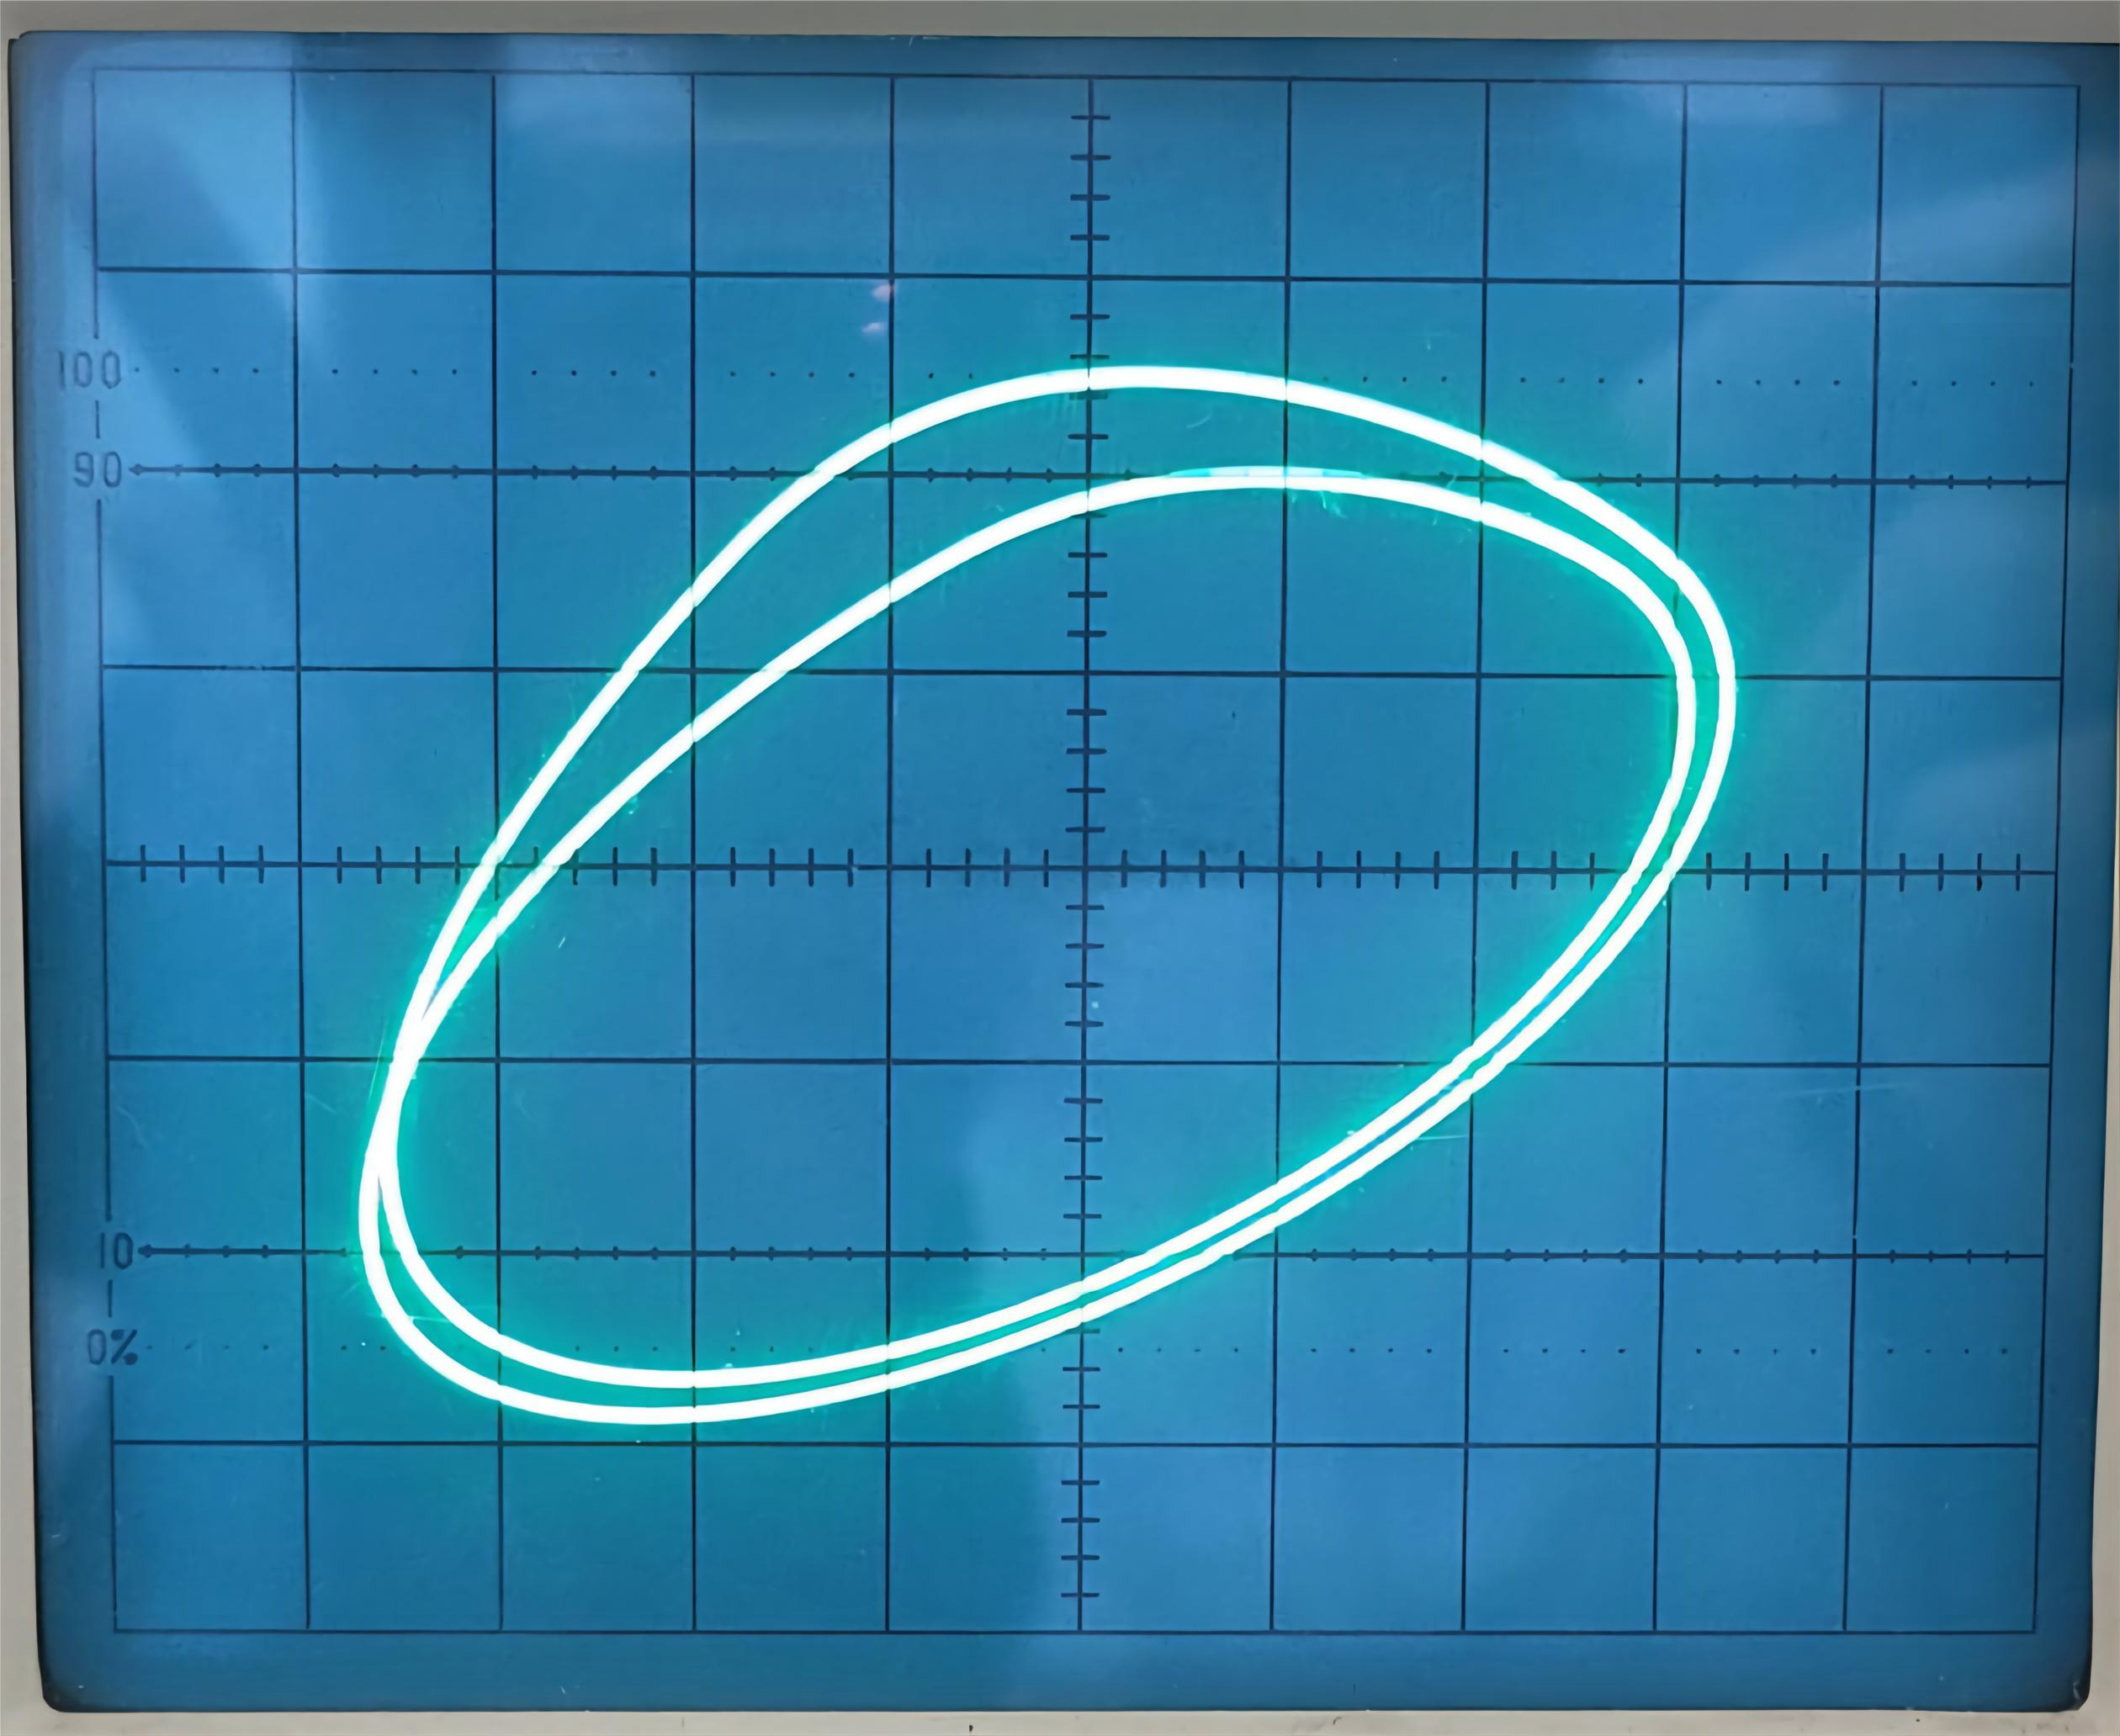
\includegraphics[width=\textwidth]{2P.png}
      \caption{2P}
    \end{subfigure}
    \hfill
    \begin{subfigure}[b]{0.3\textwidth}
      \centering
      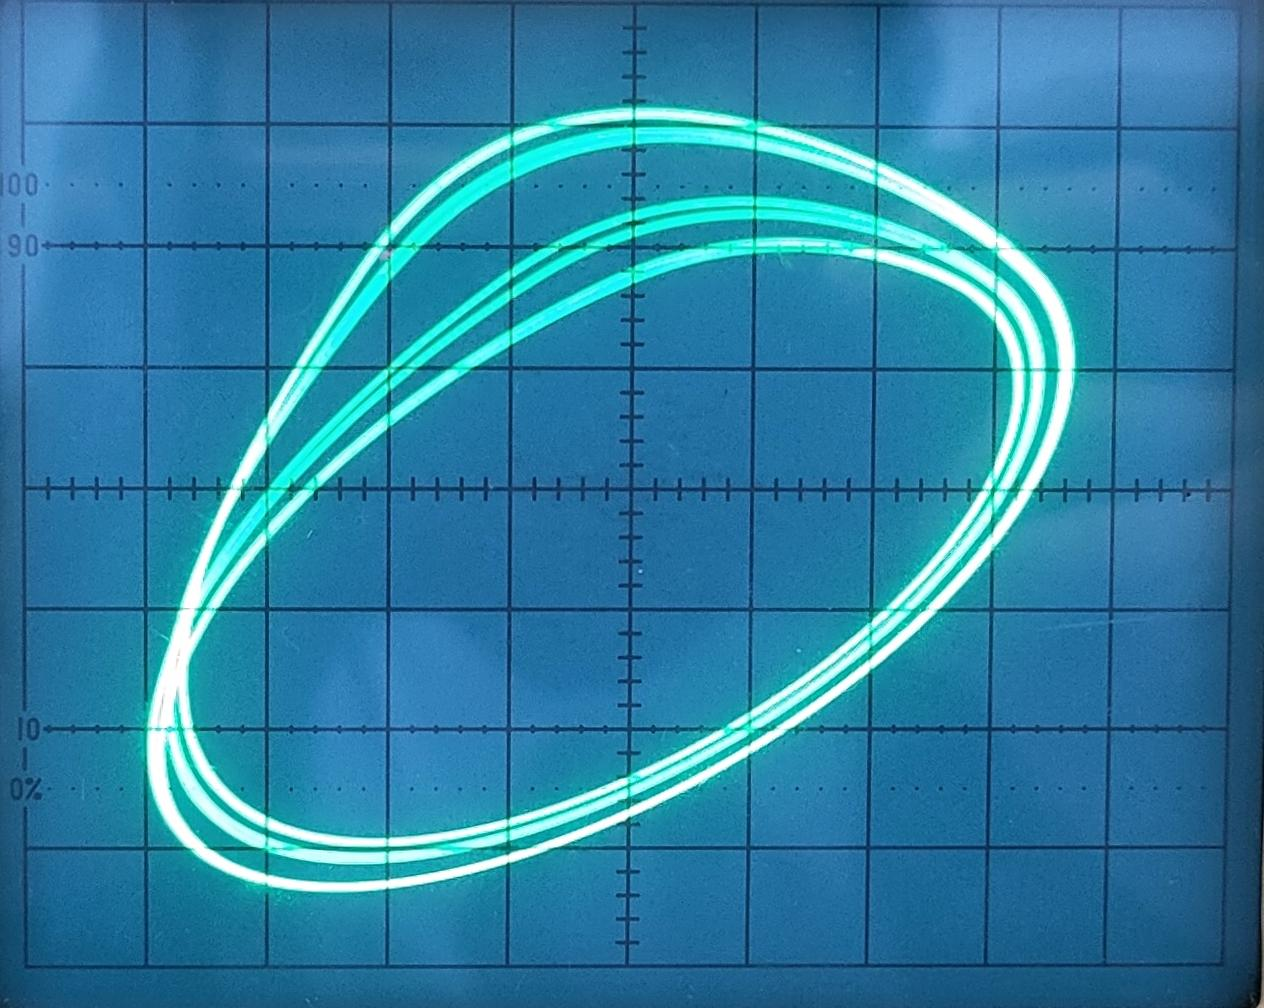
\includegraphics[width=\textwidth]{4P.png}
      \caption{4P}
    \end{subfigure}
    \\
    \begin{subfigure}[b]{0.3\textwidth}
        \centering
        \includegraphics[width=\textwidth]{6P.png}
        \caption{6P}
      \end{subfigure}
      \hfill
      \begin{subfigure}[b]{0.3\textwidth}
        \centering
        \includegraphics[width=\textwidth]{5P.png}
        \caption{5P}
      \end{subfigure}
      \hfill
      \begin{subfigure}[b]{0.3\textwidth}
        \centering
        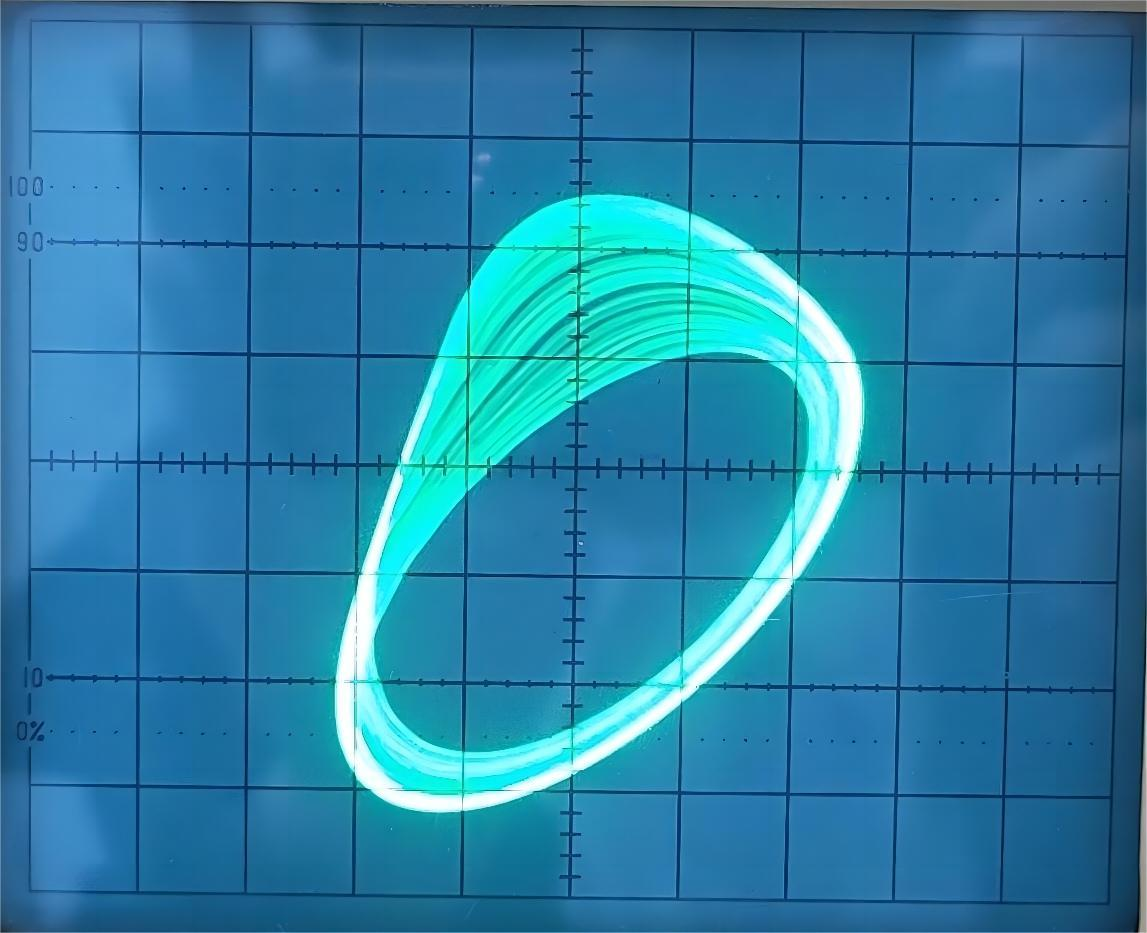
\includegraphics[width=\textwidth]{阵发混沌.png}
        \caption{阵发混沌}
      \end{subfigure}
      \\
      \begin{subfigure}[b]{0.3\textwidth}
        \centering
        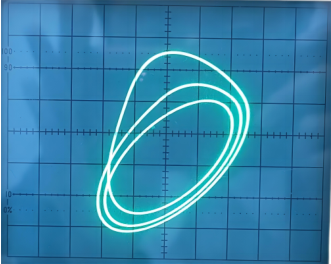
\includegraphics[width=\textwidth]{3P.png}
        \caption{3P}
      \end{subfigure}
      \hfill
      \begin{subfigure}[b]{0.3\textwidth}
        \centering
        \includegraphics[width=\textwidth]{单吸引子.png}
        \caption{单吸引子}
      \end{subfigure}
      \hfill
      \begin{subfigure}[b]{0.3\textwidth}
        \centering
        \includegraphics[width=\textwidth]{双吸引子.png}
        \caption{双吸引子}
      \end{subfigure}
    \caption{混沌运动情况}
  \end{figure}
本节用万用表测量了2P, 4P, 3P临界点有源负阻两端的交流电压, 以及单吸引子和双吸引子的典型电压, 结果如下: 
\begin{table}[H]
    \centering
    \begin{tabular}{|c|c|c|}
    \hline
         & 下叶     & 上叶     \\ \hline
    2P   & 2.7125 & 3.1089 \\ \hline
    4P   & 2.6202 & 3.0029 \\ \hline
    3P   & 2.5089 & 2.8904 \\ \hline
    单吸引子 & 1.879  & 2.22   \\ \hline
    双吸引子 & 4.85   & 4.85   \\ \hline
    \end{tabular}
    \caption{倍分岔点临界电压, 单位:V}
    \end{table}
区分上下叶, 是因为在将C1两端电压接于CH2时, 纵坐标即为有源负阻两端电压. 此时双吸引子呈纵向分布. 在双吸引子临界电压附近, 系统有概率回到上叶或下叶的稳定周期运动状态. 
两叶的临界电压值之所以不同, 可能是某种混沌特性, 也可能是万用表交流电压档未准确校零. 以上电压档均在负阻电压范围内. 

\subsection{测量费根鲍姆常数}
将$C_2$用可调电容箱代替, 选取某个可调电阻R, 记录3组倍分岔点如下: 
\begin{table}[H]
    \centering
    \begin{tabular}{|c|c|c|c|}
    \hline
           & 1      & 2      & 3      \\ \hline
    2P     & 0.0866 & 0.0604 & 0.0694 \\ \hline
    4P     & 0.0894 & 0.0634 & 0.0723 \\ \hline
    8P     & 0.0903 & 0.0641 & 0.0732 \\ \hline
    $\delta_{2}$ & 3.1111 & 4.2857 & 3.2222 \\ \hline
    \end{tabular}
    \caption{倍分岔点电容C2的值}
    \end{table}
其中, 计算费根鲍姆常数的公式是
\be{\delta_2=\frac{\mu_2-\mu_1}{\mu_3-\mu_2}}
其中$\mu_n$对应的分岔点是$2^n P$. 
由于费根鲍姆常数$\delta$是一个极限值, 而测量值只是取前几个倍周期分岔点的参数来进行计算, 所以测
量值会与实际值存在差异, 但随着 n 取值的不断增大, 计算出来的参数$\delta_n$越接近费根鲍姆常数, 相对误差
越小, 随着n→ $\infty$,相应的参数$\delta_n$ → $\delta$. 此处实验, 正是因为无法准确观测大n的倍周期分岔, 结果均一定程度偏离费根鲍姆常数. 

测量中, 判断8P轨道需要调节缩放比, 才能确定是8P, 如下图所示:
\bfig{0.7}{8P.jpg}{8P轨道缩放图}
\subsection{混沌同步}
将两个蔡氏电路调整至双吸引子的临界状态. 将其中一个蔡氏电路作为驱动系统, 另外一个蔡氏
电路作为响应系统。然后采用单向耦合电路将两个蔡氏电路连接起来, 调整 Rc 的电阻值, 观察同步现象并
得到混沌同步、准同步和去同步状态如下面三图所示: 
\begin{figure}[H]
    \centering
    \begin{subfigure}[b]{0.3\textwidth}
      \centering
      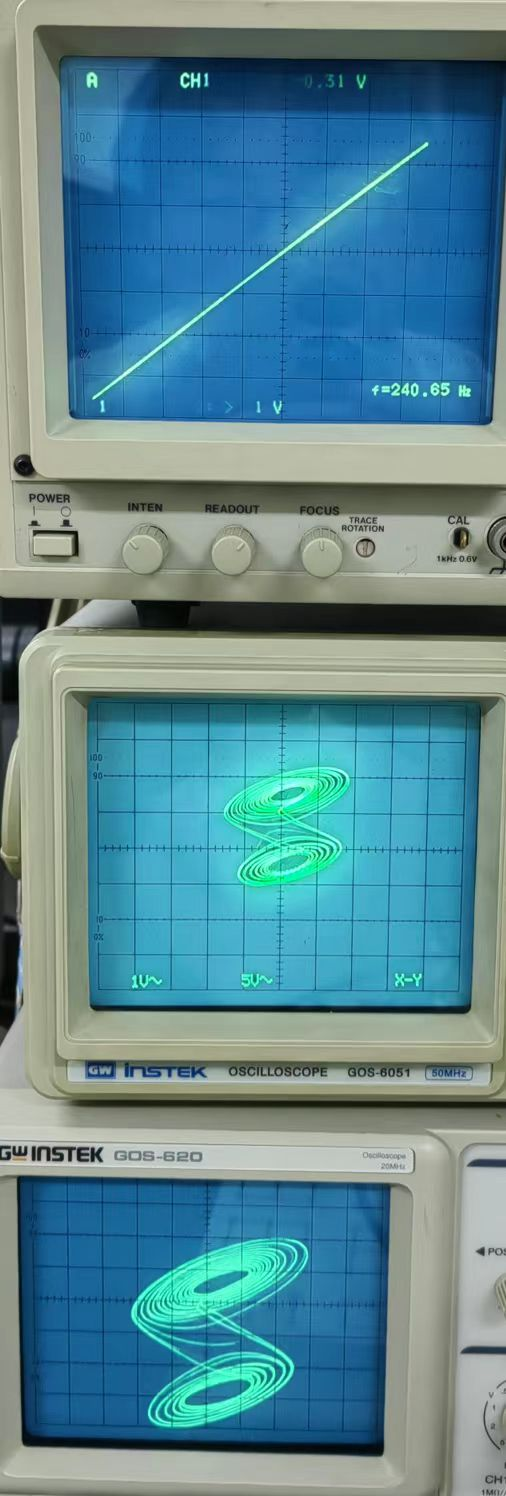
\includegraphics[width=\textwidth]{同步.jpg}
      \caption{同步}
    \end{subfigure}
    \hfill
    \begin{subfigure}[b]{0.3\textwidth}
      \centering
      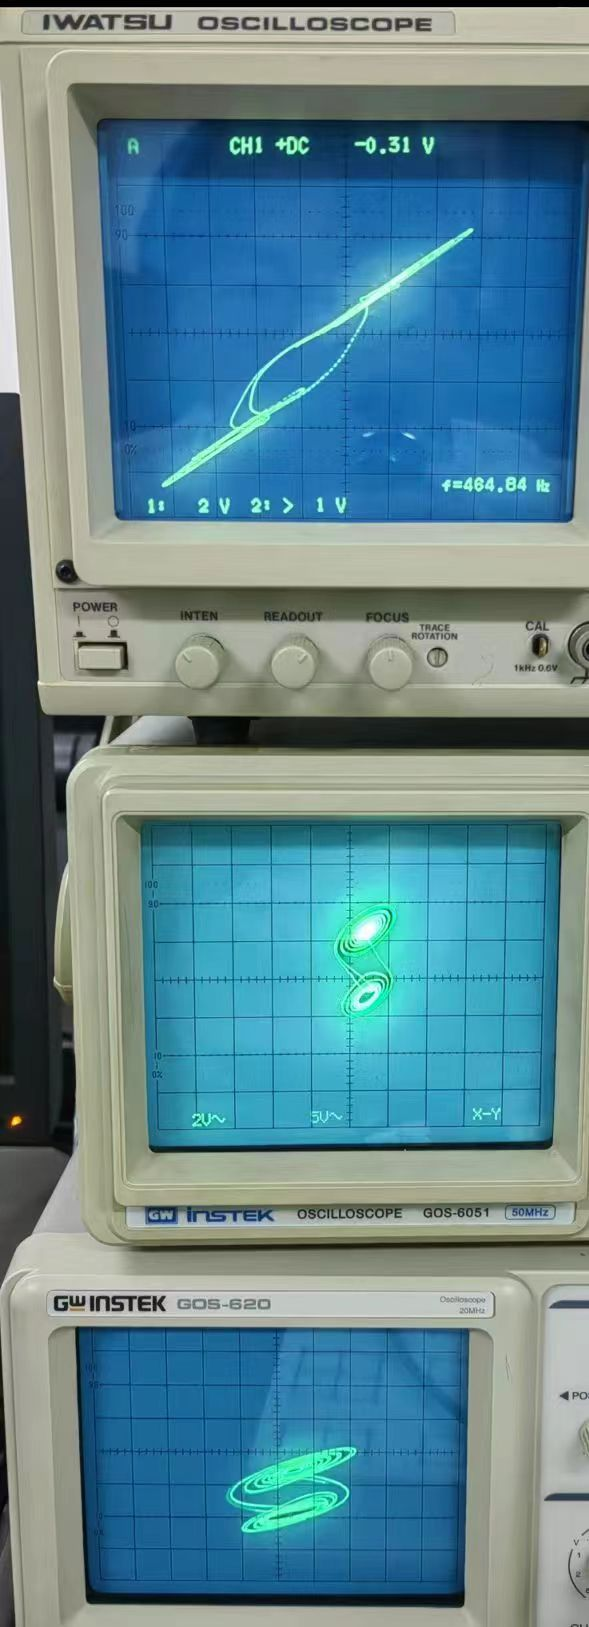
\includegraphics[width=\textwidth]{准同步.jpg}
      \caption{准同步}
    \end{subfigure}
    \hfill
    \begin{subfigure}[b]{0.3\textwidth}
      \centering
      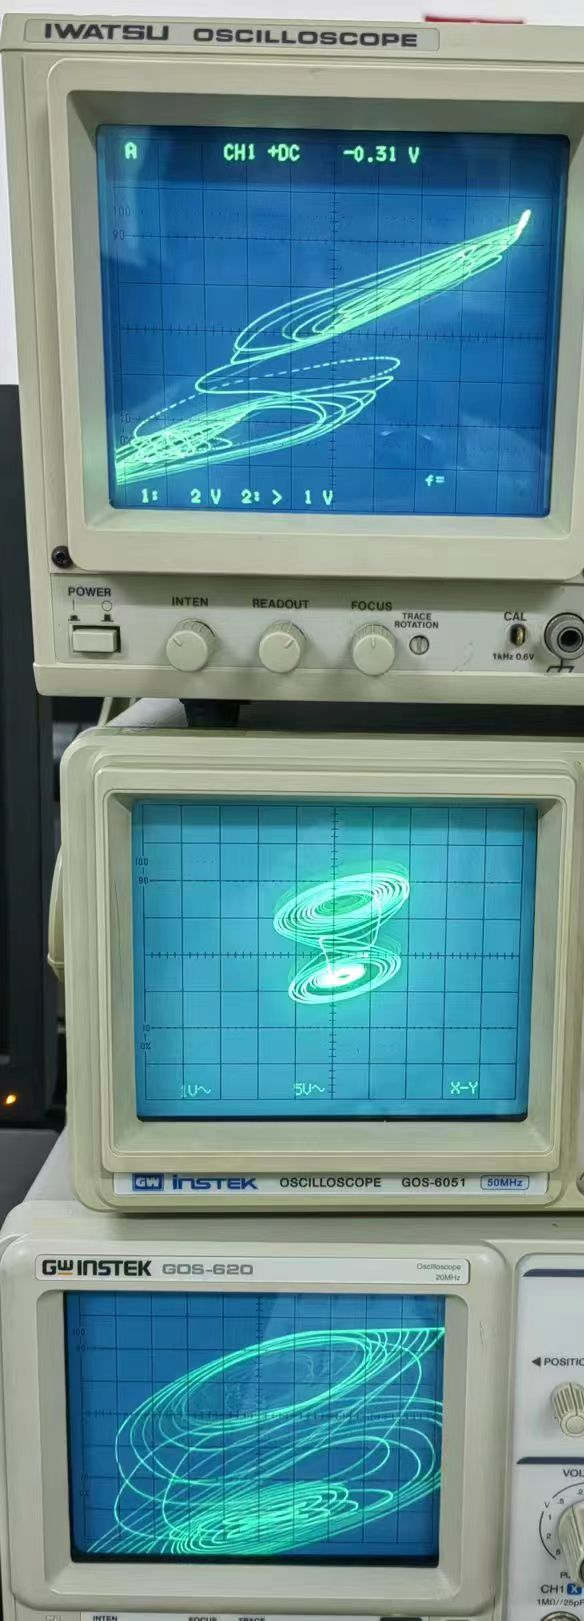
\includegraphics[width=\textwidth]{去同步.jpg}
      \caption{去同步}
    \end{subfigure}
    \caption{混沌同步示意图}
\end{figure}
图中第一行是两个电路C1两端的电压的李萨如图, 第二行是驱动电路的混沌运动, 第三行是响应电路的混沌运动. 
从同步状态到去同步状态, 是耦合电阻不断增大, 耦合电流不断减小的结果. 同步状态下, 两者呈现相位与幅值都一致的双吸引子. 准同步状态下, 相位和幅值大致相同. 去同步状态下, 相位和幅值已无太多相关性. 

即使是在去同步状态下, 尽管耦合较弱, 但仍然无法调整可变电阻R将响应电路调整至平稳的周期运动. 在更好的同步状态下时, 响应电路的参数基本不影响其运动, 完全由驱动电路的运动所控制. 

\subsection{混沌通信}
采用信号发生器信号作为
待加密信号输入加法器输入端, 驱动系统电容 C2 上的电压信号 $U_{C_2}$ 作为混沌信号连接至加法器另一输入
端, 混合得到加密信号。
将加密信号接至减法器输入端, 处于混沌同步状态的响应系统C2上的电压信号$U'_{C_2}$连接至减法器
另一输入端, 即做减法可得到解密信号, 得到解密信号. 

混沌信号如下图所示: 
\bfig{0.5}{混沌信号.jpg}{混沌信号图}
可以看出混沌信号是一系列振幅随机波和相位随机波. 

\subsubsection{正弦波信号}
以下两图图分别是加密信号, 原始信号与解密信号的对比图. 


\begin{figure}[H]
    \centering
    \begin{minipage}[t]{0.48\textwidth}
    \centering
    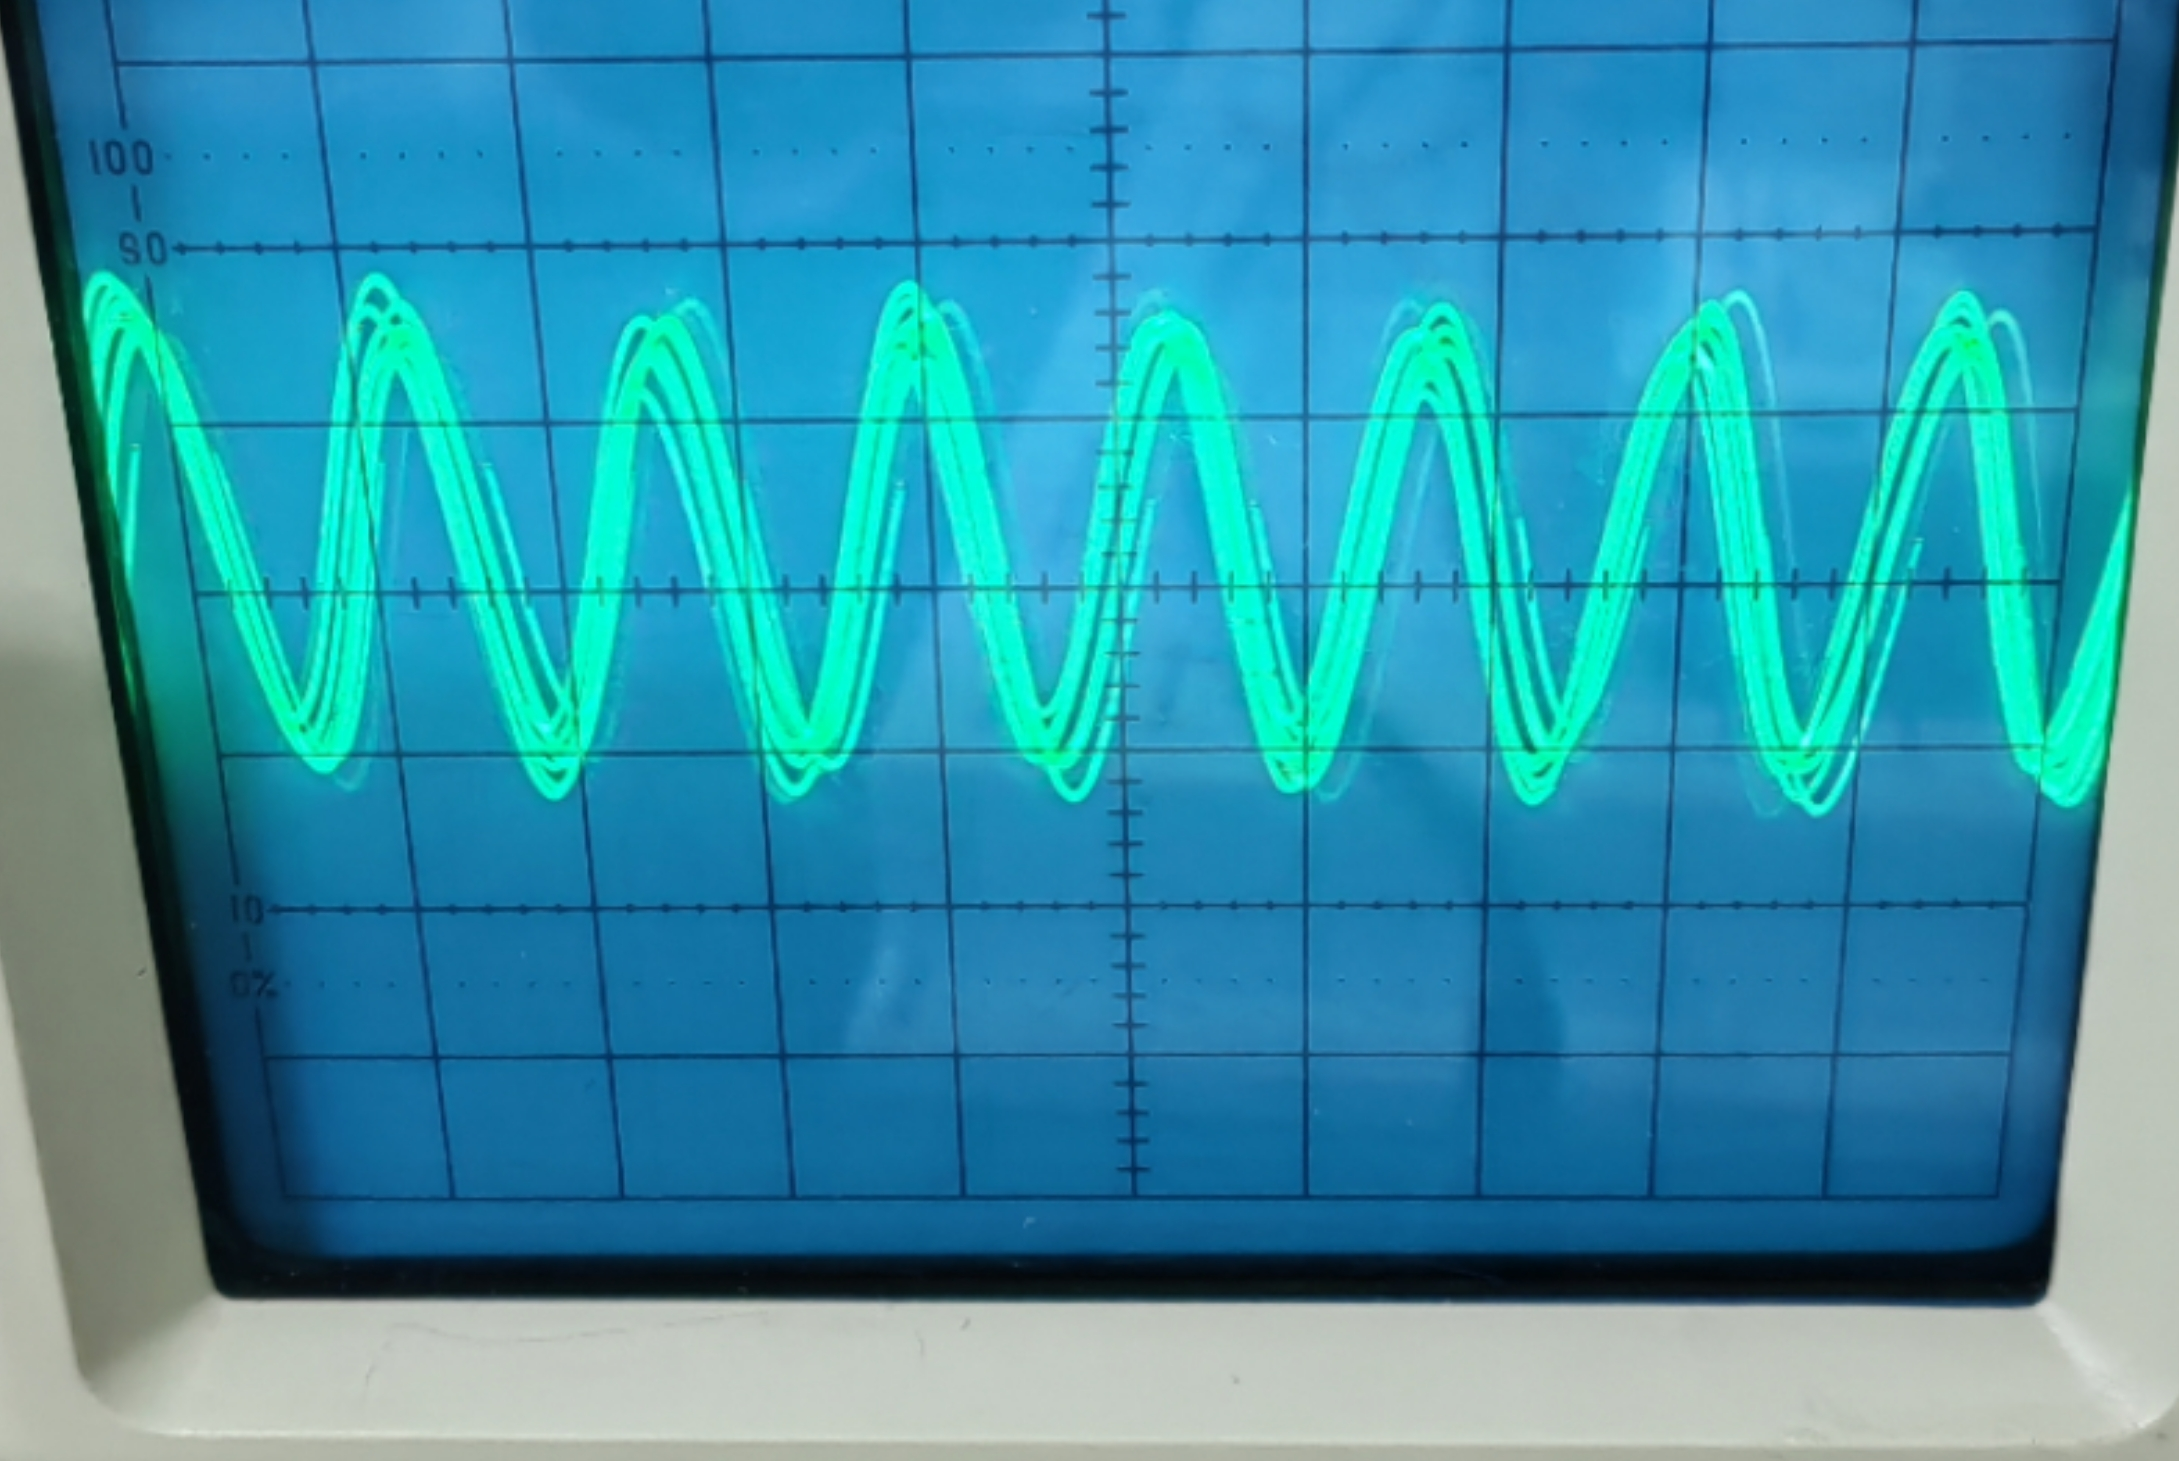
\includegraphics[width=6cm]{sin加密信号.jpg}
    \caption{加密信号}
    \end{minipage}
    \begin{minipage}[t]{0.48\textwidth}
    \centering
    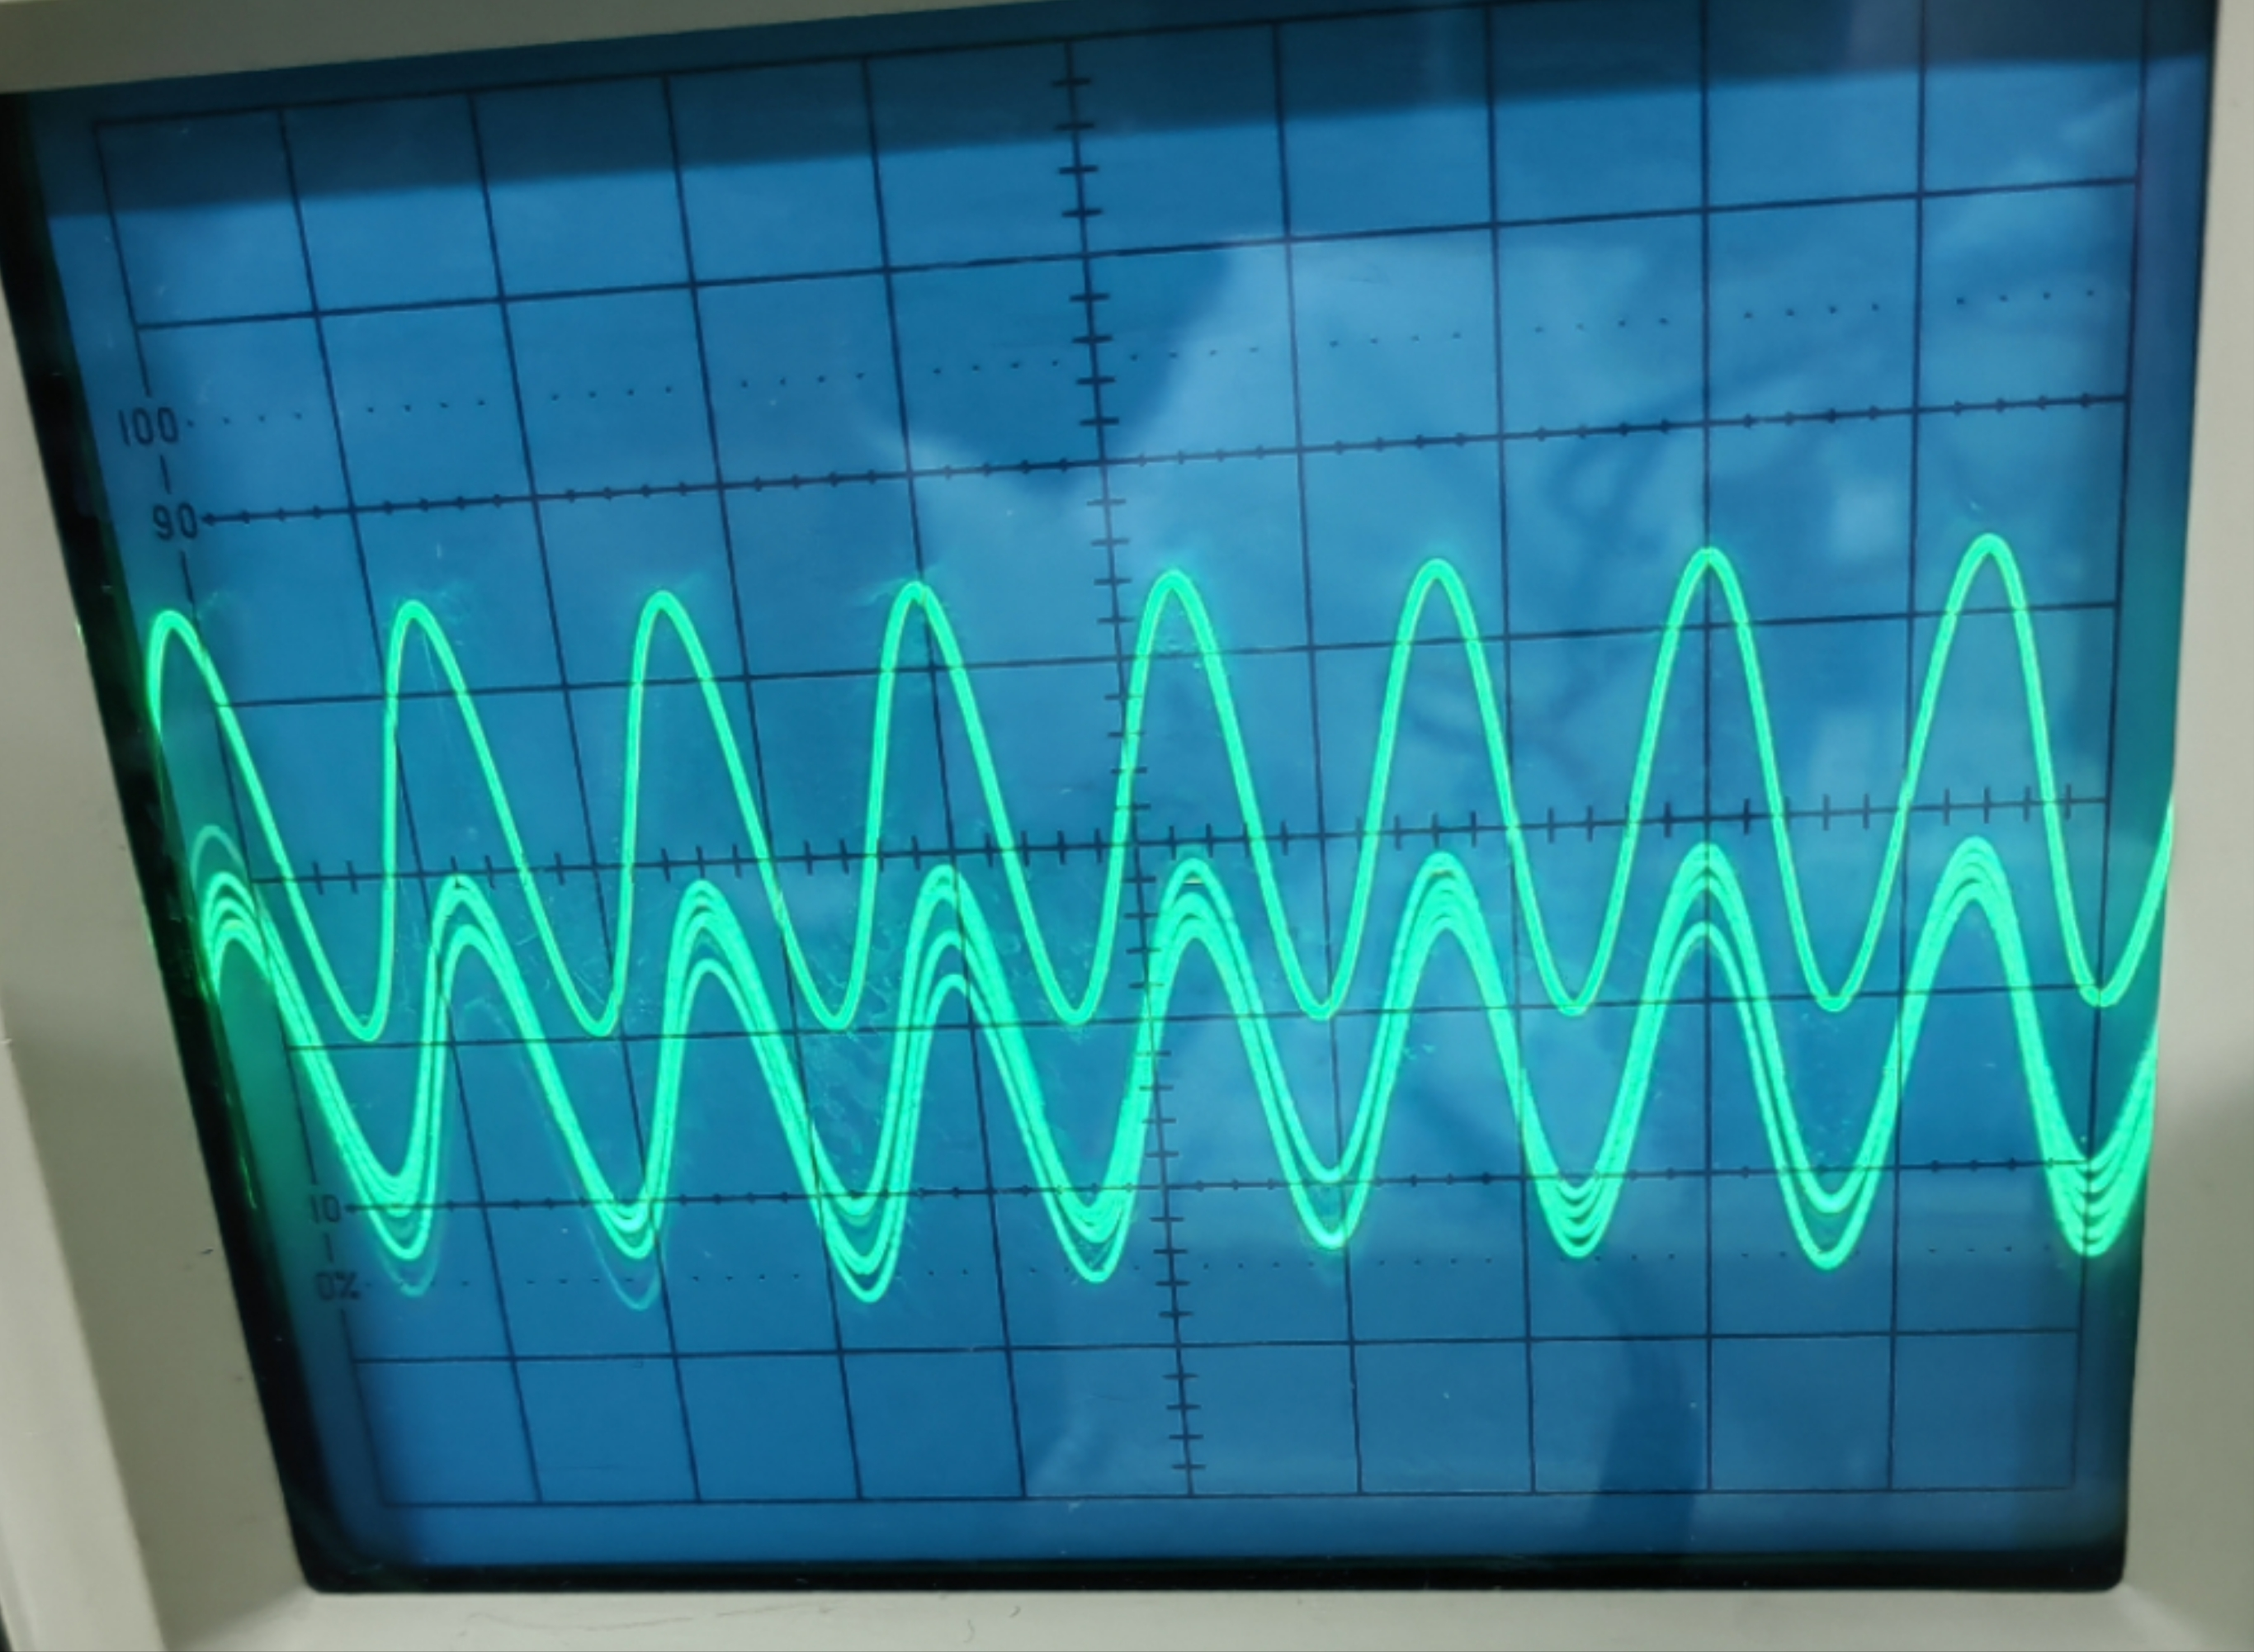
\includegraphics[width=6cm]{sin原始信号与解密信号对比.jpg}
    \caption{原始信号及解密信号}
    \end{minipage}
    \caption{正弦波通信}
    \end{figure}
    
   

可以看出, 原始信号和混沌信号叠加后, 加密信号获得了振幅随机性与波长随机性, 表现为振幅忽大忽小, 有多个峰值水平偏移. 
解密后, 从中消去了波长随机性, 表现为各峰值水平位置一致. 若用滤波器进一步滤波, 应可滤去振幅随机波. 

\subsubsection{三角波信号}
以下两图图分别是加密信号, 原始信号与解密信号的对比图.
\begin{figure}[H]
  \centering
  \begin{minipage}[t]{0.48\textwidth}
  \centering
  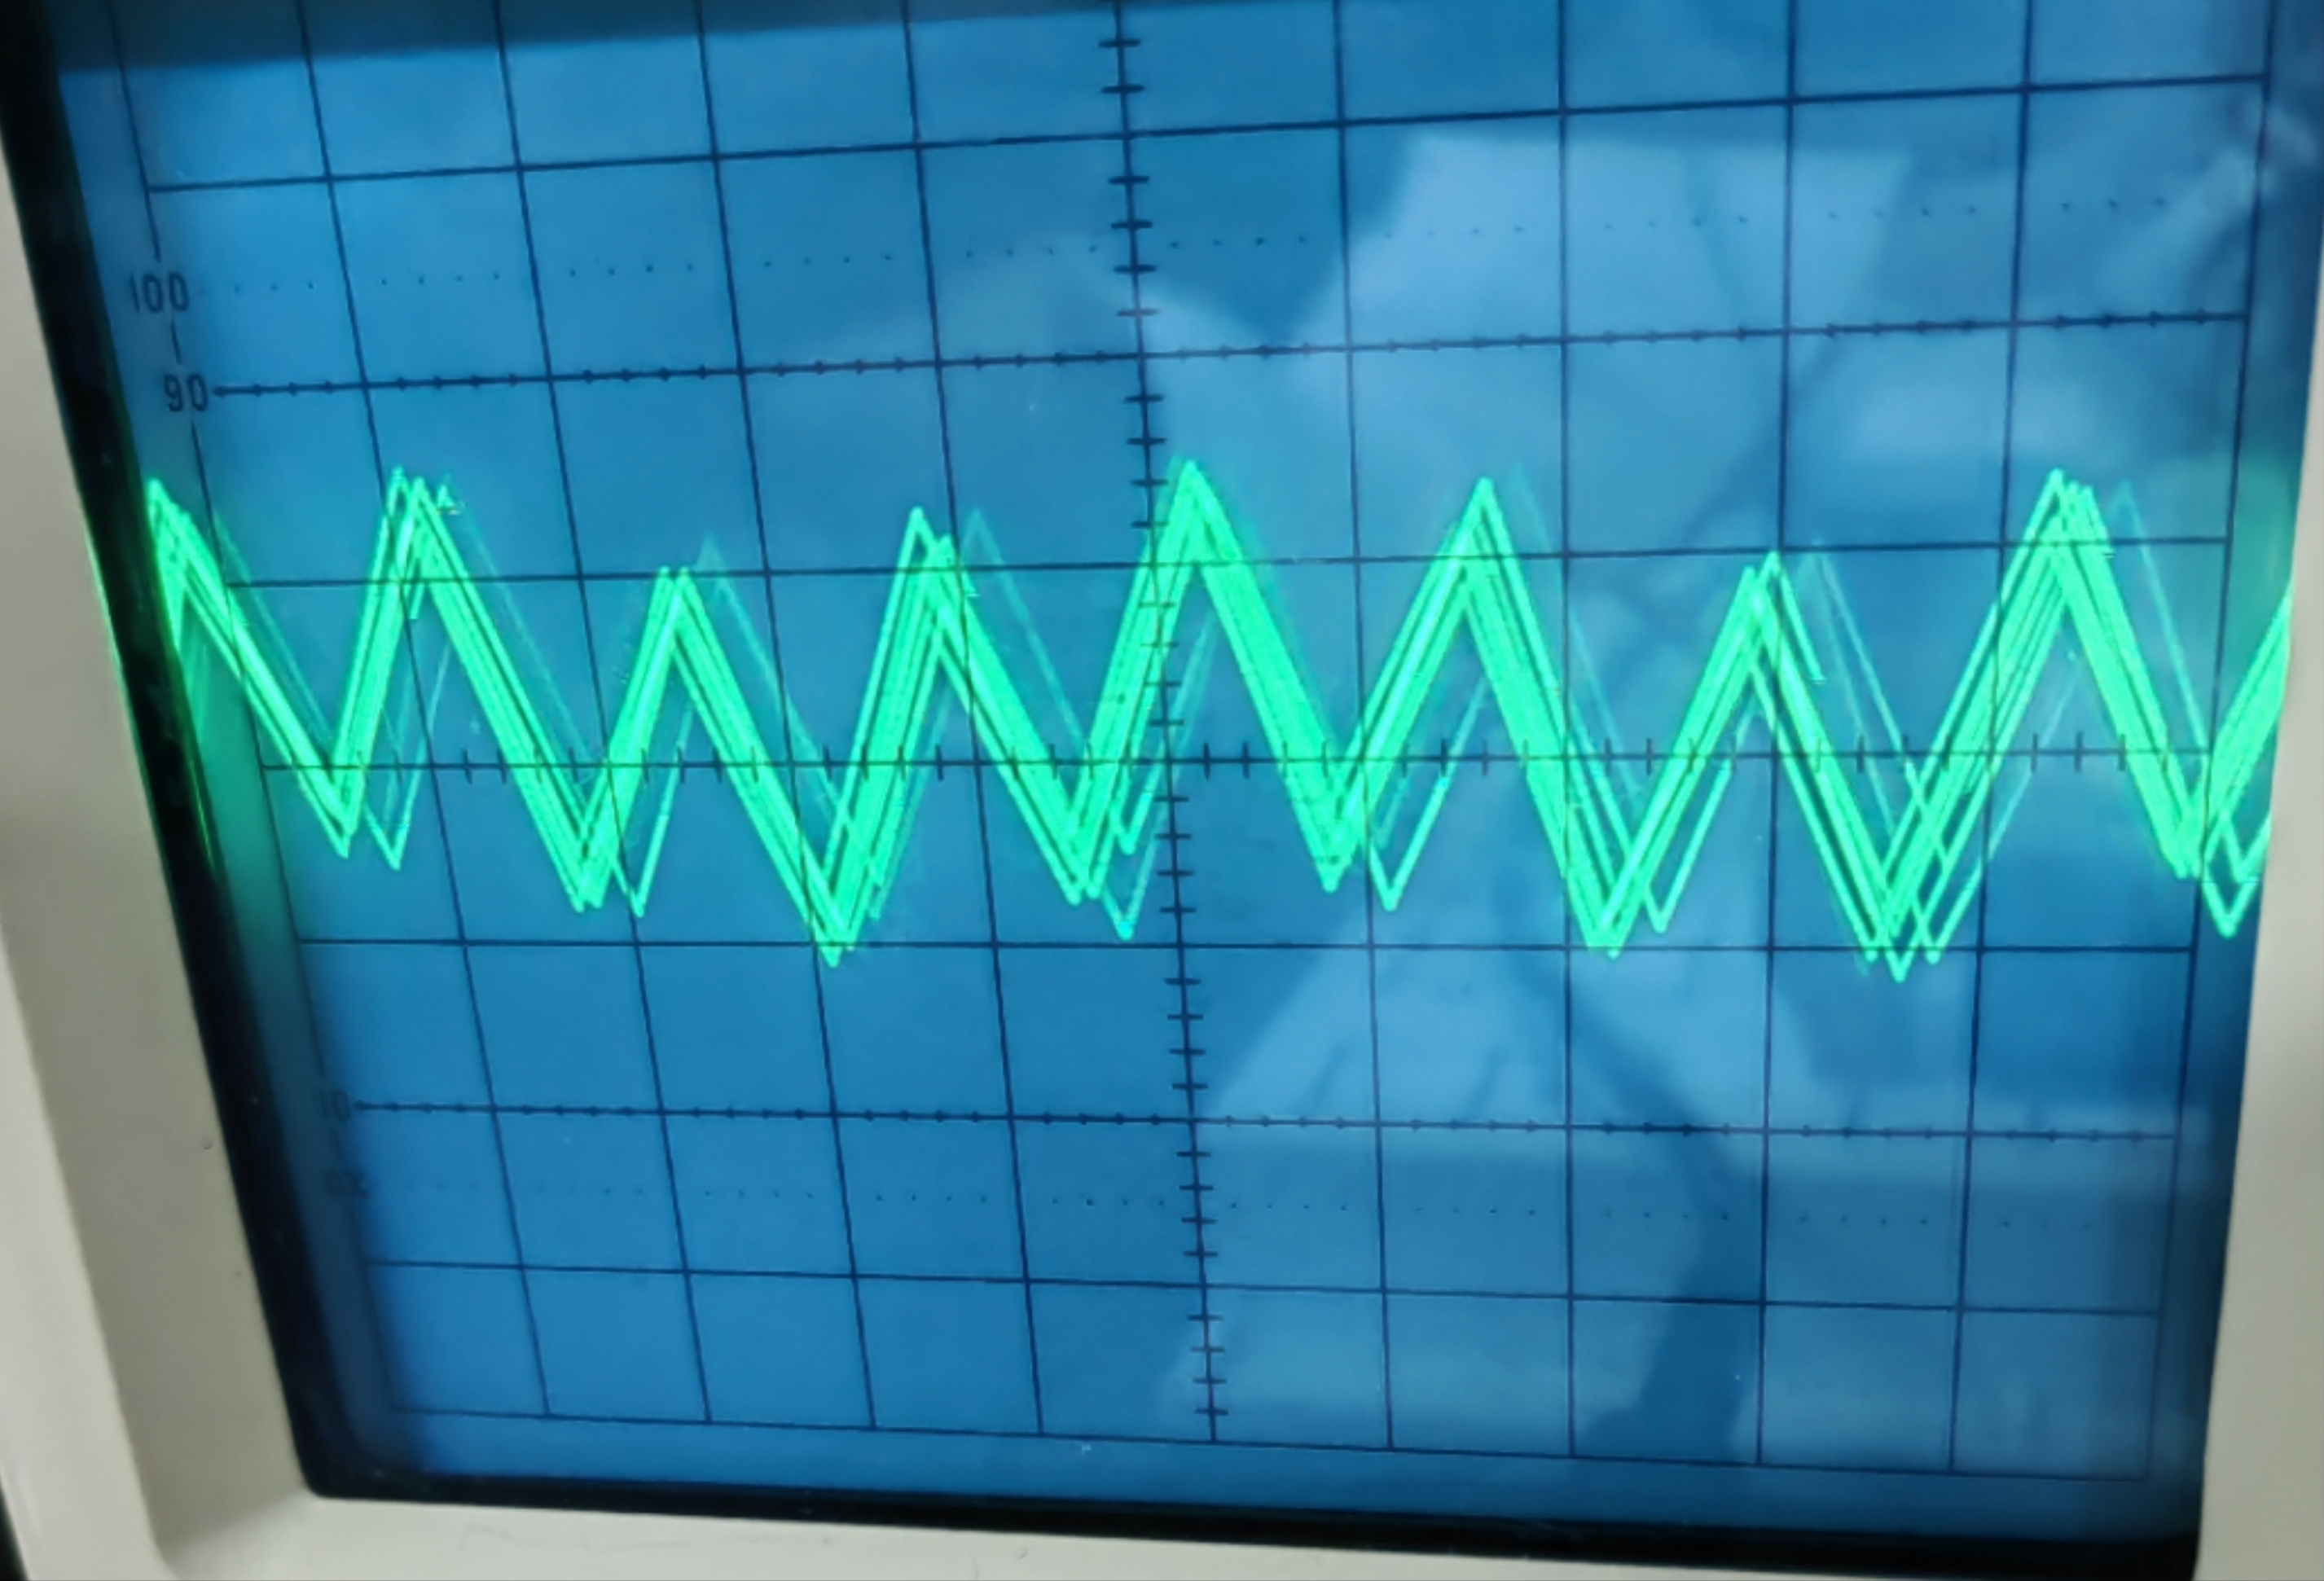
\includegraphics[width=6cm]{tri加密信号.jpg}
  \caption{加密信号}
  \end{minipage}
  \begin{minipage}[t]{0.48\textwidth}
  \centering
  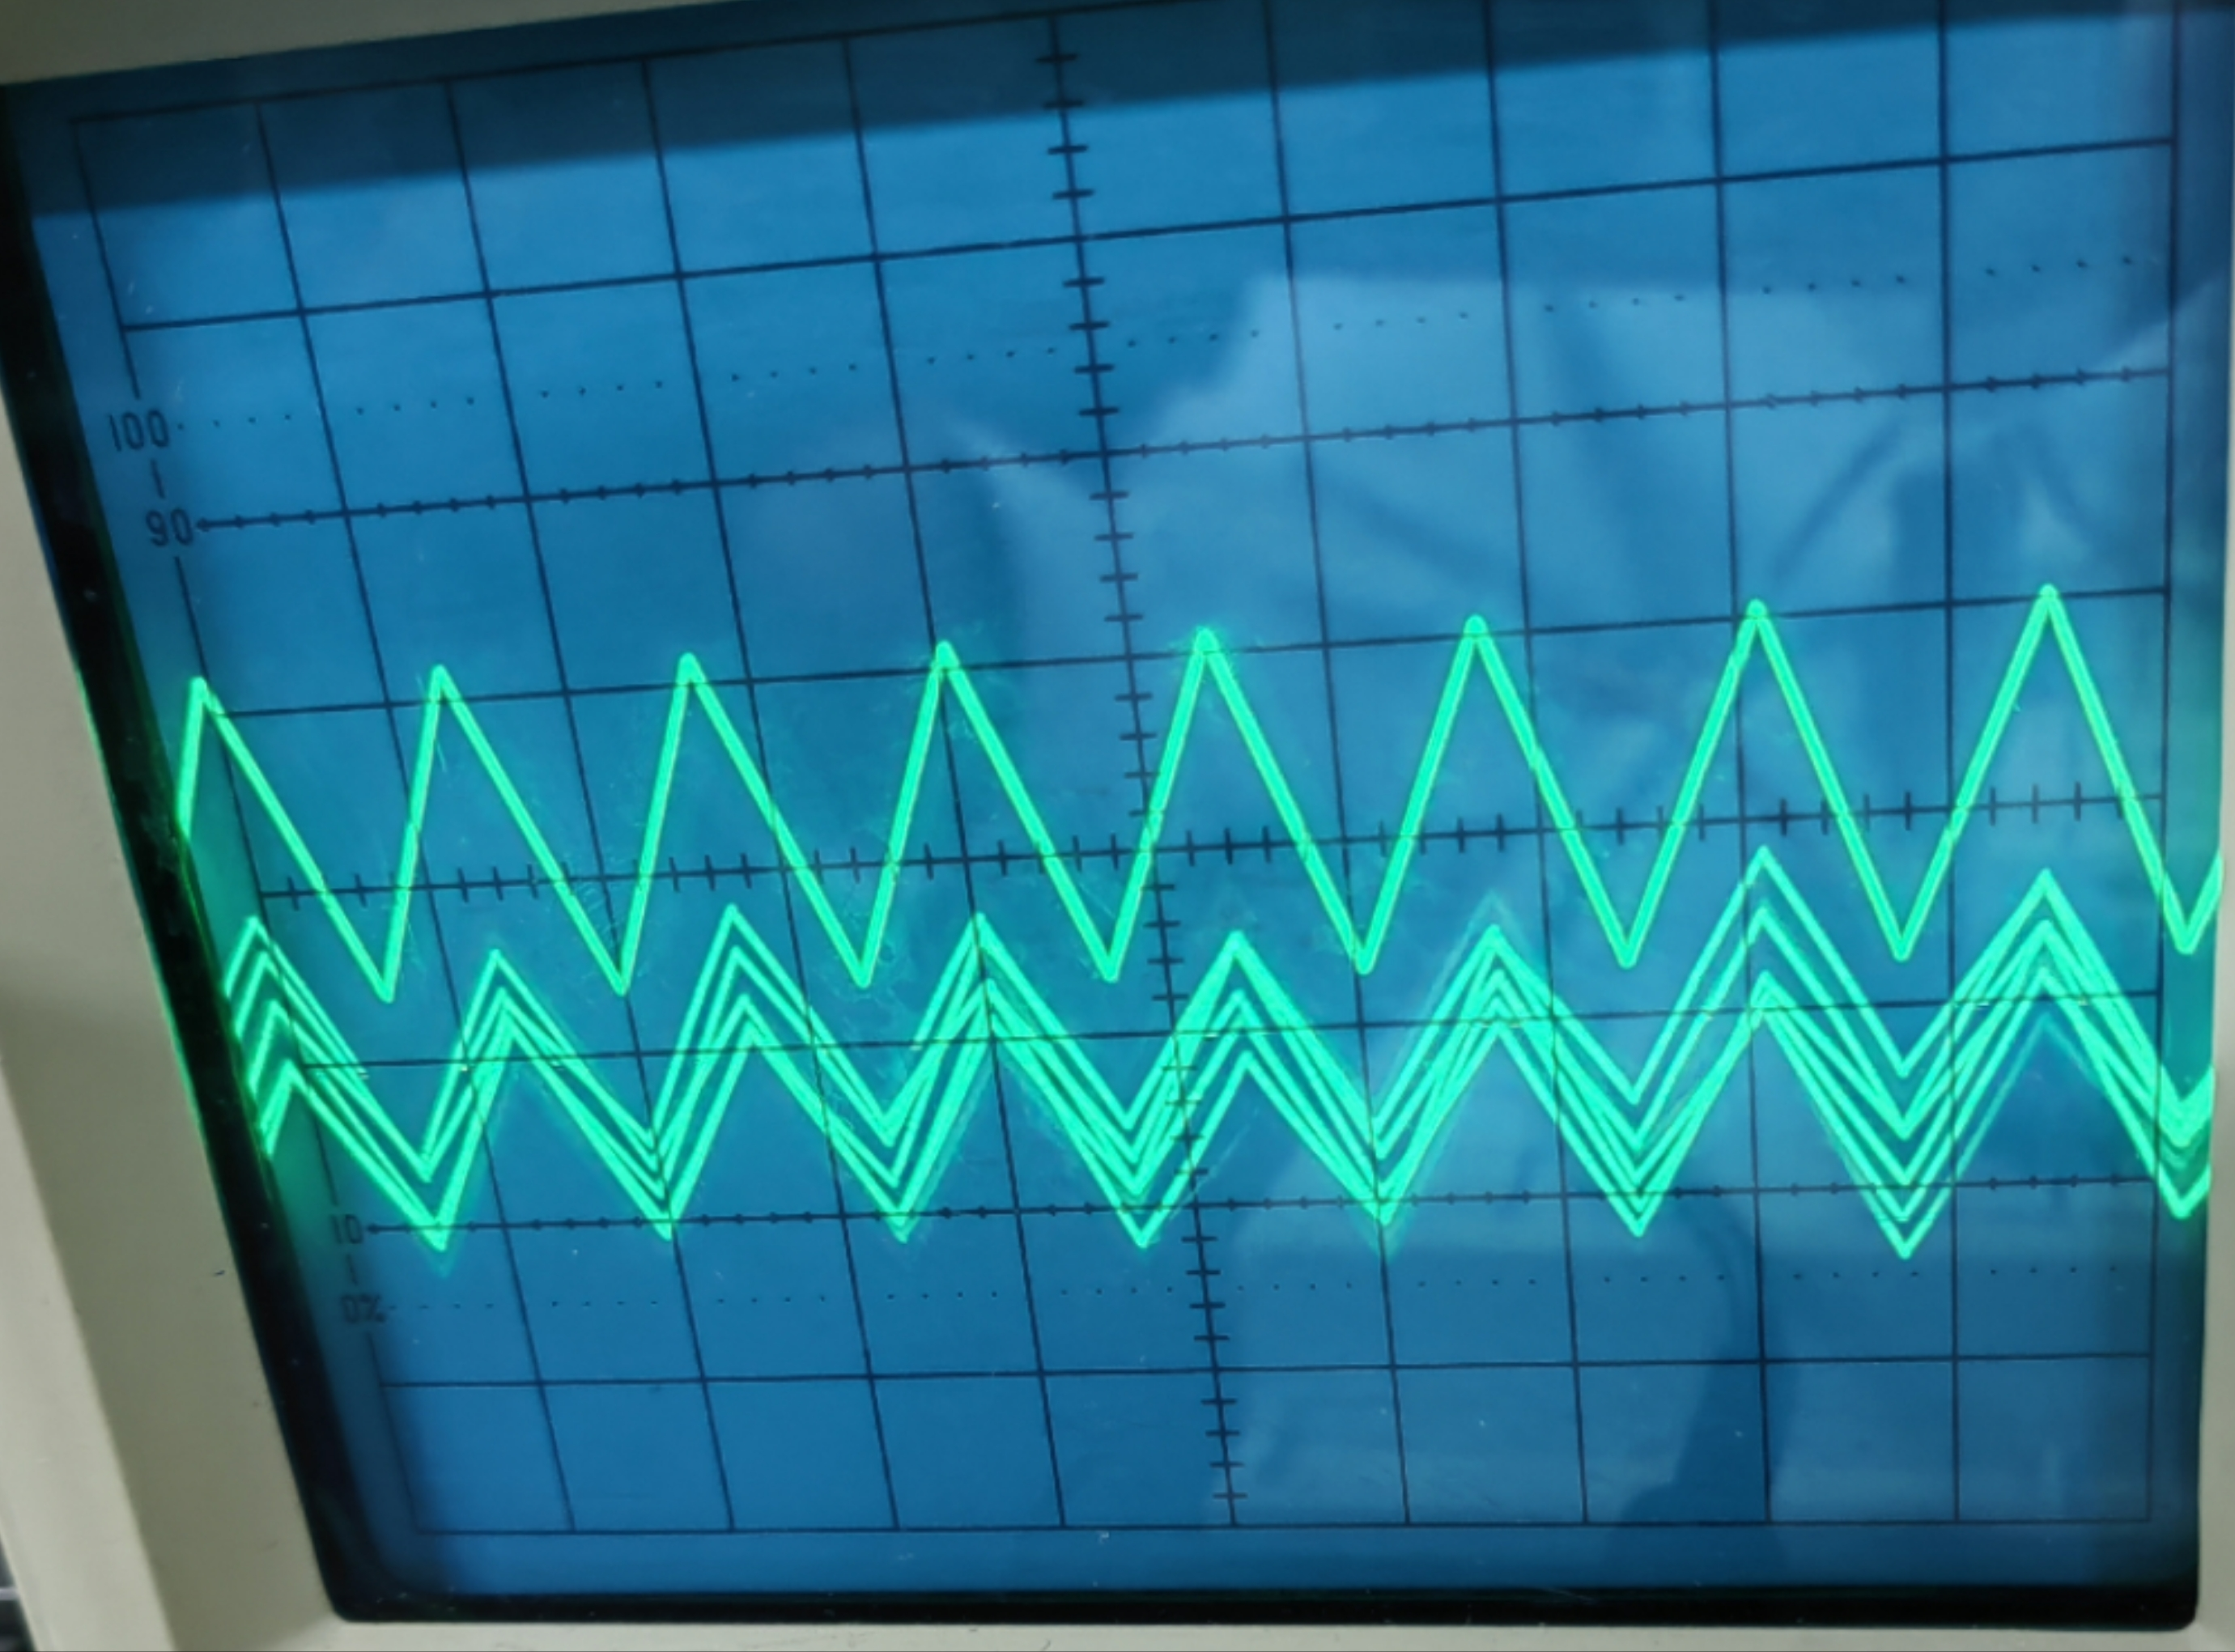
\includegraphics[width=6cm]{tri原始信号与解密信号对比.jpg}
  \caption{原始信号及解密信号}
  \end{minipage}
  \caption{正弦波通信}
  \end{figure}
结论与前面一致, 可以看出, 原始信号和混沌信号叠加后, 加密信号获得了振幅随机性与波长随机性, 表现为振幅忽大忽小, 有多个峰值水平偏移. 
解密后, 从中消去了波长随机性, 表现为各峰值水平位置一致. 若用滤波器进一步滤波, 应可滤去振幅随机波. 
\section{总结和建议}
本实验利用有源非线性负阻为主要载体, 测量并且得到了非线性负阻的I-U曲线, 并分段进行了线
性拟合, 分段得到了I-U函数关系, 并确定了负阻区。
并利用经典的非线性电路——蔡氏电路, 通过相图研究了倍周期分岔通往混沌这一典型路径, 观察系
统在该路径下的不同状态, 并因此得到了不同状态对应非线性电阻的工作区。并且利用电容箱测量了前几
个费根鲍姆参数, 并且与费根鲍姆常数理论值进行了对比, 总结了倍周期分岔通往混沌的规律。
利用隔离器在两个蔡氏电路的之间实现了单向映射, 并成功完成了混沌同步的实验, 观察了两个系统
之间的混沌同步、准同步、去同步现象, 并总结了混沌同步的特征。
最后在混沌同步电路的基础上, 进行了混沌加密通信实验。模拟了加密通信的过程, 并且初步接触了
信号的加密和解密的过程, 对混沌系统的用途有了更深的理解。


\end{document}